\documentclass[10pt]{beamer}

\usetheme[progressbar=frametitle]{metropolis}
\usepackage{appendixnumberbeamer}

\usepackage{booktabs}
\usepackage[scale=2]{ccicons}

\usepackage{pgfplots}
\usepgfplotslibrary{dateplot}

\usepackage{xspace}
\newcommand{\themename}{\textbf{\textsc{metropolis}}\xspace}

\usepackage{listings}

\usepackage{graphicx}
\usepackage{multirow}
\usepackage{makecell} % for more vertical space in cells
\setcellgapes{5pt}

\usepackage{amsmath}
\DeclareMathOperator*{\argmin}{arg\,min}

\usepackage[T1]{fontenc}
\usepackage[utf8]{inputenc}

\title{Fraud detection \\ using Cost Sensitive methods}
\author{Patryk Wielopolski}
\institute{Wrocław Univeristy of Technology and Science \\ Koło Naukowe Statystyki Matematycznej ,,Gauss''}
\date{}

\begin{document}
    \newcommand{\htx}{h_{\theta}(\boldsymbol{x_i})}

    \newenvironment{talign}
    {\align}
    {\endalign}
    
    \newenvironment{talign*}
    {\csname align*\endcsname}
    {\endalign}

\maketitle

\begin{frame}{Fraud}
    Fraud - the crime of getting money by deceiving people.
    
    \bigskip
    
    Examples of frauds:
    \begin{itemize}
        \item Using a stolen credit card
        \item Overstating the cost of compensation
        \item Reporting event which never happened
        \item ...
    \end{itemize}{}
    
    \nocite{CSCCFD}
    \nocite{ICCFD}
    \nocite{alej2015ensemble}
\end{frame}{}

\begin{frame}{Fraud detection techniques}
    Fraud detection techniques:
    \begin{itemize}
        \item Probability models
        \item Anomaly detection
        \item Data mining
        \item Expert rules systems
        \item Pattern recognition
        \item Machine learning
    \end{itemize}{}
\end{frame}{}

\begin{frame}{Problems}
    Problems which occurs during modeling:
    \begin{itemize}
        \item Insufficient standard metrics 
        \item Highly imbalanced dataset (class disproportion up to 1:1000)
        \item Labels distortions
    \end{itemize}
\end{frame}{}

\section{Classification of methodology for classification problems}

\begin{frame}{Standard methodology}
    Standard methodology for classification problem:
    \begin{itemize}
        \item Standard models:
            \begin{itemize}
                \item Logistice regression
                \item Decision Tree
                \item Random Forest
                \item XGBoost
            \end{itemize}
        \item Standard metrics:
            \begin{itemize}
                \item Accuracy
                \item Precision
                \item Recall
                \item F1 Score
            \end{itemize}{}
    \end{itemize}
\end{frame}{}

\begin{frame}{Confusion matrix}
    \begin{center}
        \makegapedcells
        \begin{tabular}{cc|cc}
            \multicolumn{2}{c}{}
                        &   \multicolumn{2}{c}{Prediction} \\
                &       &   Fraud &   Non-Fraud              \\ 
                \cline{2-4}
            \multirow{2}{*}{\rotatebox[origin=c]{90}{True}}
                & Fraud   & TP   & FN                 \\
                & Non-Fraud   & FP   & TN                \\ 
                \cline{2-4}
        \end{tabular}
    \end{center}
    
    $$ \text{Accuracy} = \frac{TP + TN}{TP + FP + FN + TN} $$
    $$ \text{Precision} = \frac{TP}{TP + FP} $$
    $$ \text{Recall}= \frac{TP}{TP + FN} $$
    $$ \text{F1 Score} = 2 \cdot \frac{\text{Precision} \cdot \text{Recall}}{\text{Precision} + \text{Recall}} $$
\end{frame}

\begin{frame}{Cost Sensitive Methodology}
    Cost Sensitive Methodology:
    \begin{itemize}
        \item Cost dependent classification:
            \begin{itemize}
                \item Threshold optimization
                \item Bayesian Minimum Risk
            \end{itemize}{}
        \item Cost sensitive training:
            \begin{itemize}
                \item Cost Sensitive Logistic Regression
                \item Cost Sensitive Decision Tree
            \end{itemize}
        \item Cost sensitive metrics
            \begin{itemize}
                \item Total cost
                \item Savings
            \end{itemize}{}
    \end{itemize}
\end{frame}{}

\begin{frame}{Cost matrix}
    \begin{center}
        \makegapedcells
        \begin{tabular}{cc|cc}
            \multicolumn{2}{c}{}
                        &   \multicolumn{2}{c}{Prediction} \\
                &       &   Fraud &   Non-Fraud              \\ 
                \cline{2-4}
            \multirow{2}{cc}{\rotatebox[origin=c]{90}{True}}
                & Fraud   & C_{TP_{i}}   & C_{FN_{i}}                 \\
                & Non-Fraud   & C_{FP_{i}}   & C_{TN_{i}}                \\ 
                \cline{2-4}
        \end{tabular}
    \end{center}
    
    $$ \text{Cost}(f(\boldsymbol{x}_{i}^{*})) = y_i (c_i C_{TP_i} + (1-c_i)C_{FN_i}) + (1-y_i)(c_i C_{FP_i} + (1-c_i)C_{TN_i})$$

    \begin{itemize}
        \item $\boldsymbol{x}_{i}^{*} = [\boldsymbol{x}_i, C_{TP_{i}}, C_{FP_{i}}, C_{FN_{i}}, C_{TN_{i}}]$ - features vector for i-th observation extended by classification cost
        \item $C_{\cdot}$ - classification cost for i-th observation
        \item $f(\cdot)$ - predictive model
        \item $y_i$ - true label for i-th observation
        \item $c_i$ - prediction for i-th observation
    \end{itemize}{}
    
\end{frame}{}

\begin{frame}{Cost Sensitive metrics}
    Cost sensitive metrics:
    $$ \text{Total cost}(f(\boldsymbol{S})) = \sum_{i=1}^{N}\text{Cost}(f(\boldsymbol{x}_{i}^{*})) $$
    $$ \text{Savings} = \frac{\text{Cost}_{l}(\boldsymbol{S}) - \text{Cost}(f(\boldsymbol{S}))}{\text{Cost}_{l}(\boldsymbol{S})} $$

    \begin{itemize}
        \item $ \boldsymbol{S} $ - data set
        \item $ \text{Cost}_l = min\{\text{Cost}(f_{0}(\boldsymbol{S}), \text{Cost}(f_{1}(\boldsymbol{S})\} $
        \item $ f_{a}(\boldsymbol{S}) = \boldsymbol{a} $ where $a \in \{0,1\}$
    \end{itemize}{}
    
\end{frame}{}

\section{Cost Sensitive Modeling}

\begin{frame}{Threshold Optimization}
    We are looking for threshold $th$ such that
    $$ \argmin_{th \in [0,1]} \text{Total cost}(\boldsymbol{C}, \boldsymbol{P}) $$
    Where 
    \begin{itemize}
        \item $ \boldsymbol{C} = (c_i)_{i=1}^n $ - vector of true labels
        \item $ \boldsymbol{P} = (p_i > th)_{i=1}^n $ - vector of binary outcomes
    \end{itemize}{}
\end{frame}{}

\begin{frame}{Bayesian Minimum Risk}
    Risk associated with predictions:
    
    $$ R(p_f|x) = L(p_f|y_f)P(p_f|x) + L(p_f|y_l)P(y_l|x) $$
    $$ R(p_l|x) = L(p_l|y_l)P(p_l|x) + L(p_l|y_f)P(y_f|x) $$
    
    Classification threshold:
    
    $$ R(p_f|x) \leq R(p_l|x)$$
    
    Where:
    
    \begin{itemize}
        \item $P(p_f|x)$, $P(p_l|x)$ - estimated probability of fraud/legimate transaction
        \item $L(p_{i}|y_{j})$ and $i,j \in \{l,f\}$ - loss function
    \end{itemize}{}

\end{frame}{}

\begin{frame}{Bayesian Minimum Risk}
    Exact formula:
    
    $$ P(p_f|x) \ge \frac{L(p_f|y_l) - L(p_l|y_l)}{L(p_l|y_f) - L(p_f|y_f) - L(p_l|y_l) + L(p_f|y_l)}$$
    
    After reformulation:
    
    $$ p \ge \frac{C_{FP} - C_{TN}}{C_{FN} - C_{TP} - C_{TN} + C_{FP}}$$
    
\end{frame}{}

\begin{frame}{Cost Sensitive Logistic Regression}
    Formulation of standard Logistic Regression:
    
    $$ \hat{p} = P(y=1|\boldsymbol{x_i}) = h_{\theta}(\boldsymbol{x_i}) = g\left(\sum_{j=1}^k \theta^{(j)}x_i^{(j)} \right) $$
    
    Where loss function is defined:
    
    $$ J(\theta) = \frac{1}{N} \sum_{i=1}^N J_i(\theta) $$
    
    Where:
    
    \begin{itemize}
        \item $ \displaystyle g(z) = \frac{1}{(1+e^{-z})} $
        \item $ \displaystyle J_i(\theta) = -y_i log(h_{\theta}(\boldsymbol{x_i})) - (1-y_i) log(1 - h_{\theta}(\boldsymbol{x_i})) $
    \end{itemize}{}
    
    
\end{frame}{}

\begin{frame}{Cost Sensitive Logistic Regression}
    Standard costs:
    $$
    J_i(\theta) \approx \left\{
        \begin{array}{rl}
             0, &\mbox{if $y_i \approx \htx$}, \\
             \infty, &\mbox{if $y_i \approx (1 - \htx)$}.
        \end{array}{}
    \right.
    $$
    
    Thus
    
    $$ C_{TP_i} = C_{TN_i} \approx 0 $$
    $$ C_{FP_i} = C_{FN_i} \approx \infty $$
    
\end{frame}{}

\begin{frame}{Cost Sensitive Logistic Regression}
    Actual costs:
    
     $$
    J^c_i(\theta)=\left\{
        \begin{array}{rl}
            C_{TP_i}, &\mbox{if $y_i = 1$ and $\htx \approx 1$}, \\
            C_{TN_i}, &\mbox{if $y_i = 0$ and $\htx \approx 0$}, \\
            C_{FP_i}, &\mbox{if $y_i = 0$ and $\htx \approx 1$}, \\
            C_{FN_i}, &\mbox{if $y_i = 1$ and $\htx \approx 0$}.
        \end{array}
    \right.
    $$
    
    Cost sensitive loss function:
    \begin{talign*}
        J^c(\theta) &= \frac{1}{N} \sum_{i=1}^{N} \bigg( y_i \Big( \htx C_{TP_i} + (1 - \htx)C_{FN_i} \Big) \\
        &+ (1-y_i) \Big( \htx C_{FP_i} + (1 - \htx)C_{TN_i} \Big) \bigg)
    \end{talign*}
\end{frame}{}

\begin{frame}{Cost Sensitive Decision Tree}

    Standard impurity measures:
    \begin{itemize}
        \item Misclassification: $I_m(\pi_1) = 1 - \max(\pi_1, 1 - \pi_1)$
        \item Entropy: $I_e(\pi_1) = -\pi_1 \log(\pi_1) - (1 - \pi_1) \log (1 - \pi_1)$
        \item Gini: $I_g(\pi_1) = 2 \pi_1 (1 - \pi_1)$
    \end{itemize}{}
    
    Cost Sensitive impurity measure:
    \begin{itemize}
        \item $I_c(\mathcal{S}) = min \left\{ Cost(f_0(\mathcal{S})), Cost(f_1(\mathcal{S})) \right\}$
    \end{itemize}{}
    
    Where:
    \begin{itemize}
        \item $\pi_1 = \frac{|\mathcal{S}_{1}|}{|\mathcal{S}|}$ - percentage of positive class
        \item $\mathcal{S}$ - set of samples
    \end{itemize}{}
\end{frame}{}

\section{Experiment}

\begin{frame}{Experiment description}
    Data set:
        \begin{itemize}
            \item Credit Card Fraud Detection Dataset 
            \item 284,807 transactions with 492 frauds
            \item Class imbalance approx. 1:600 (0.172\% fraud transactions)
        \end{itemize}{}
    Data split:
        \begin{itemize}
            \item Training: 50\%
            \item Validation: 17\%
            \item Test: 33\%
        \end{itemize}{}
\end{frame}

\begin{frame}{Cost matrix for the experiment}
    Cost matrix:
    
    \begin{center}
        \makegapedcells
        \begin{tabular}{cc|cc}
            \multicolumn{2}{c}{}
                        &   \multicolumn{2}{c}{Prediction} \\
                &       &   Fraud &   Non-Fraud              \\ 
                \cline{2-4}
            \multirow{2}{cc}{\rotatebox[origin=c]{90}{True}}
                & Fraud   & C_{TP_{i}} = C_a   & C_{FN_{i}} = \text{Amt}_i   \\
                & Non-Fraud   & C_{FP_{i}} = C_a & C_{TN_{i}} = 0                \\ 
                \cline{2-4}
        \end{tabular}
    \end{center}
    
    \begin{itemize}
        \item $\text{Amt}_i$ - Value of transaction
        \item $C_a$ - Administrative cost
    \end{itemize}{}
    
    Decision threshold for Bayesian Minimum Risk:
    
    $$ p \ge \frac{C_a}{\text{Amt}_i} $$
\end{frame}

\begin{frame}{Results - Savings}
    \begin{figure}
        \centering
        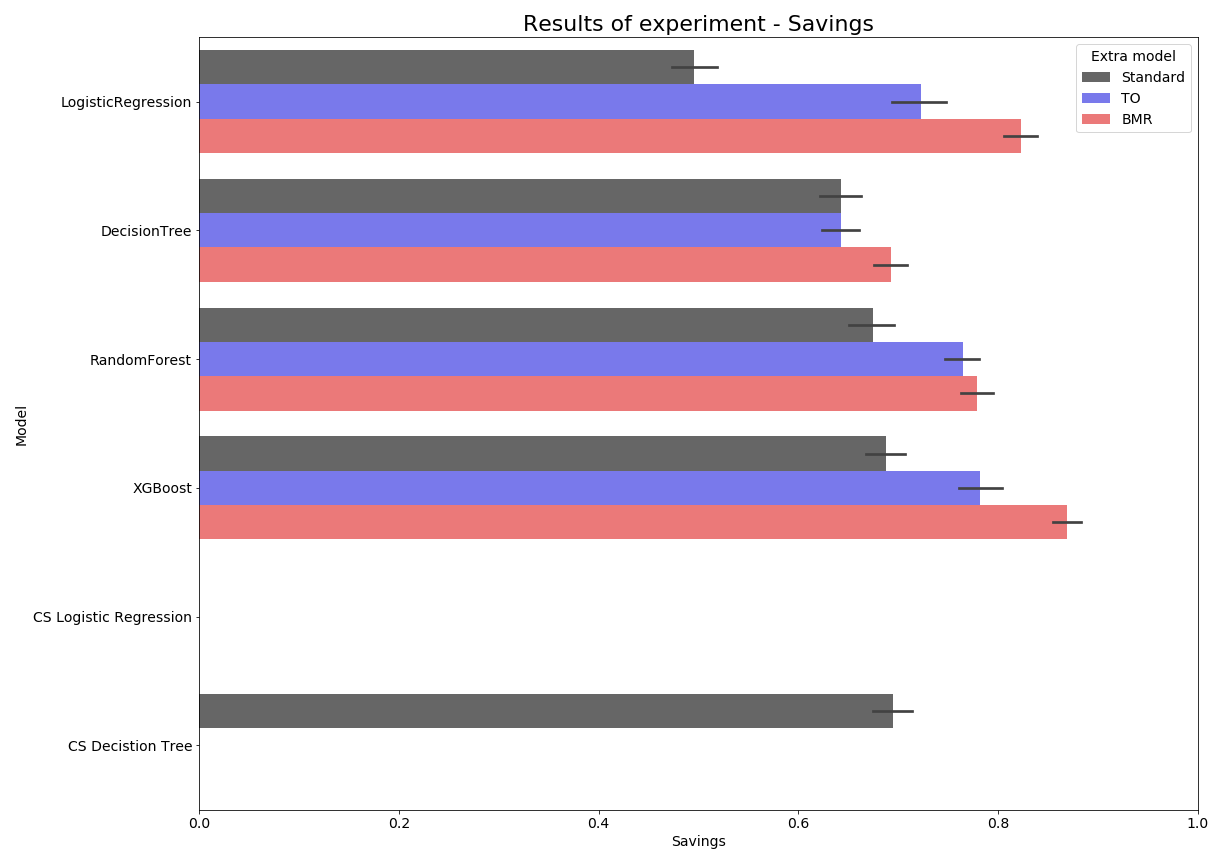
\includegraphics[width=0.9\linewidth,height=\textheight,keepaspectratio]{Config1-Savings.png}
        \caption{Results of the experiment for $C_a = 1$ and Saving metric.}
    \end{figure}
\end{frame}

\begin{frame}{Results - F1 Score}
    \begin{figure}
        \centering
        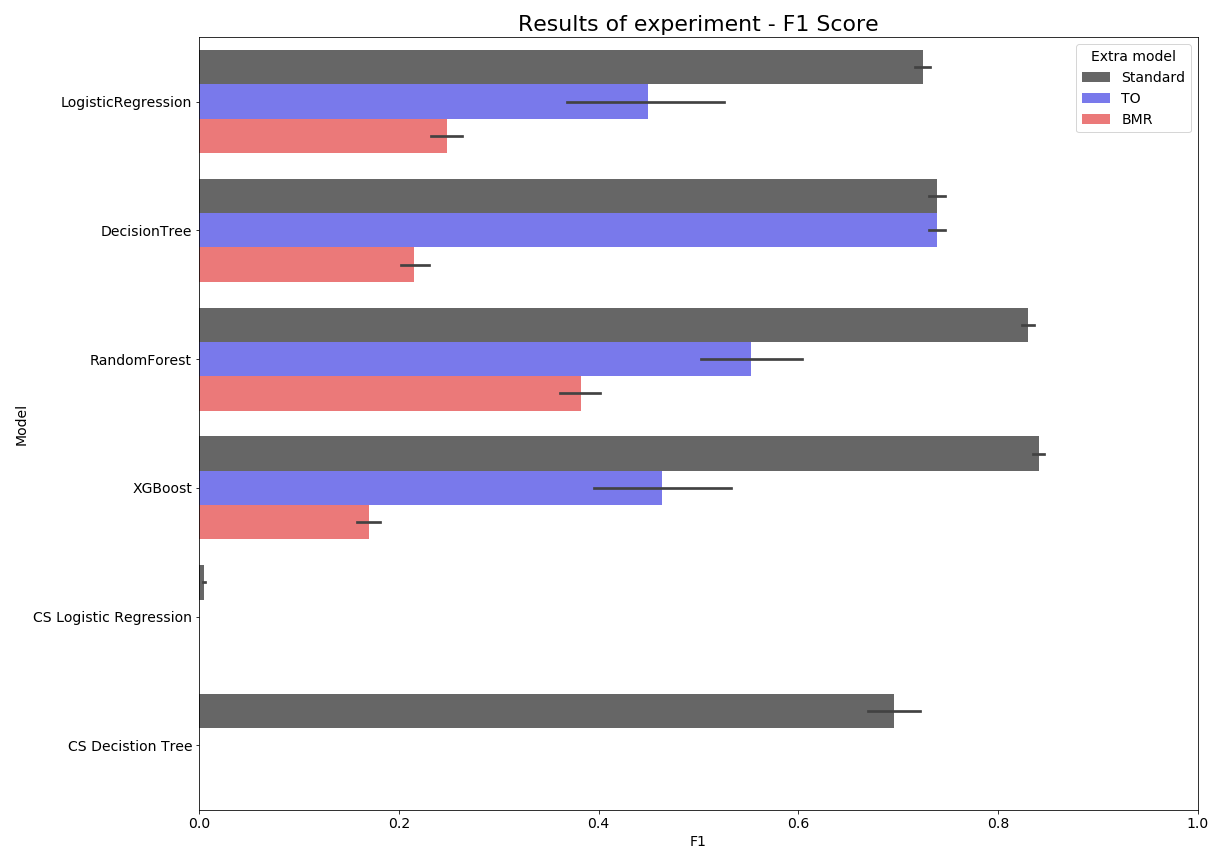
\includegraphics[width=0.9\linewidth,keepaspectratio]{Config1-F1.png}
        \caption{Results of the experiment for $C_a = 1$ and F1 Score metric.}
    \end{figure}
\end{frame}

\begin{frame}{Conclusions}
    Conclusions:
    \begin{itemize}
        \item Threshold Optimization and Bayesian Minimum Risk improves results for Savings metric, \pause
        \item But unfortunately almost always worsens the results for F1 Score metric, \pause
        \item And this leads to trade-off between cost and precision/recall. \pause
        \item Cost Sensitive training may be good choice when Savings and F1 Score are simultaneously important.
    \end{itemize}{}
\end{frame}{}

\begin{frame}{Future work}
    Future work:
    \begin{itemize}
        \item Conducting the experiment in respect to different administrative cost.
        \item Extension of the used models with Cost Sensitive Ensembles and other boosting models (e.g. LightGMB, CatBoost).
        \item Extension of the experiment with under/over-sampling methods.
        \item Defining custom loss function (similarly to Logistic Regression) for boosting algorithms.
    \end{itemize}{}
\end{frame}{}

\begin{frame}[allowframebreaks]{References}

  \bibliography{references}
  \bibliographystyle{abbrv}

\end{frame}

{\setbeamercolor{palette primary}{fg=white, bg=black}
\begin{frame}
    \centering
    {\Large Thanks for your attention!}
    
    \bigskip
    
    Questions?
\end{frame}
}

\end{document}

